%%%%%%%%%%%%%%%%%%%%%%%%%%%%%%%%%%%%%%%%%%%%%%%%%%%%%%%%%%%%%%%%%%%%%%%%%%%%%%%
% Chapter 'Absorption - Water - ionic liquid [DEMA][OMs]'
%%%%%%%%%%%%%%%%%%%%%%%%%%%%%%%%%%%%%%%%%%%%%%%%%%%%%%%%%%%%%%%%%%%%%%%%%%%%%%%
\subsection{Ionic liquid [DEMA][OMs]}
%
%%%%%%%%%%%%%%%%%%%%%%%%%%%%%%%%%%%%%%%%%%%%%%%%%%%%%%%%%%%%%%%%%%%%%%%%%%%%%%%
%%%%%%%%%%%%%%%%%%%%%%%%%%%%%%%%%%%%%%%%%%%%%%%%%%%%%%%%%%%%%%%%%%%%%%%%%%%%%%%
\subsubsection{NrtlFixedDg - ID 1}
%
\begin{tabular}[l]{|lp{11.5cm}|}
\hline
\addlinespace

\textbf{Sorbent:} & ionic liquid \\
\textbf{Subtype:} & [DEMA][OMs] \\
\textbf{Refrigerant:} & Water \\
\textbf{Equation:} & NrtlFixedDg \\
\textbf{ID:} & 1 \\
\textbf{Reference:} & Römich, Christiane; Merkel, Nina C.; Valbonesi, Alessandro; Schaber, Karlheinz; Sauer, Sven; Schubert, Thomas J. S. (2012): Thermodynamic Properties of Binary Mixtures of Water and Room-Temperature Ionic Liquids. Vapor Pressures, Heat Capacities, Densities, and Viscosities of Water + 1-Ethyl-3-methylimidazolium Acetate and Water + Diethylmethylammonium Methane Sulfonate. In: J. Chem. Eng. Data 57 (8), S. 2258–2264. DOI: 10.1021/je300132e. \\
\textbf{Comment:} & None \\

\addlinespace
\hline
\end{tabular}
\newline

\textbf{Equation and parameters:}
\newline
%
Pressure $p$ in $\si{\pascal}$ is calculated depending on molar fraction of refrigerant in the liquid phase $x_1$ in $\si{\mole\per\mole}$, temperature $T$ in $\si{\kelvin}$, and vapor pressure $p_\mathrm{sat,1}$ in $\si{\pascal}$ by:
%
\begin{equation*}
\begin{split}
p &=& \gamma_1 x_1 p_\mathrm{sat,1} & \quad\text{, and} \\
\gamma_1 &=& \exp \left( x_2^2 \left( \tau_{21} \left( \frac{G_{21}}{x_1 + x_2 G_{21}} \right) ^2 + \tau_{12} \frac{G_{12}}{\left( x_2 + x_1 G_{12} \right) ^2}\right) \right) & \quad\text{, and} \\
G_{12} &=& \exp \left( -\alpha_{12} \tau_{12} \right) & \quad\text{, and} \\
G_{21} &=& \exp \left( -\alpha_{21} \tau_{21} \right) & \quad\text{, and} \\
\tau_{12} &=& \nicefrac{\Delta g_{12}}{R T} & \quad\text{, and} \\
\tau_{21} &=& \nicefrac{\Delta g_{21}}{R T} & \quad\text{, and} \\
x_2 &=& 1 - x_1  & \quad\text{.} \\
\end{split}
\end{equation*}
%
The parameters of the equation are:
%
\begin{longtable}[l]{lll|lll}
\toprule
\addlinespace
\textbf{Par.} & \textbf{Unit} & \textbf{Value} &	\textbf{Par.} & \textbf{Unit} & \textbf{Value} \\
\addlinespace
\midrule
\endhead

\bottomrule
\endfoot
\bottomrule
\endlastfoot
\addlinespace

$\alpha_{12}$ & - & 7.086200000e-01 & $\alpha_{21}$ & - & 7.086200000e-01 \\
$\Delta g_{12}$ & $\si{\joule\per\mole}$ & -1.051400000e+03 & $\Delta g_{21}$ & $\si{\joule\per\mole}$ & -5.039900000e+03 \\

\addlinespace\end{longtable}

\textbf{Validity:}
\newline
Equation is approximately valid for $303.15 \si{\kelvin} \leq T \leq 353.15 \si{\kelvin}$.
\newline

\textbf{Visualization:}
%
\begin{figure}[!htp]
{\noindent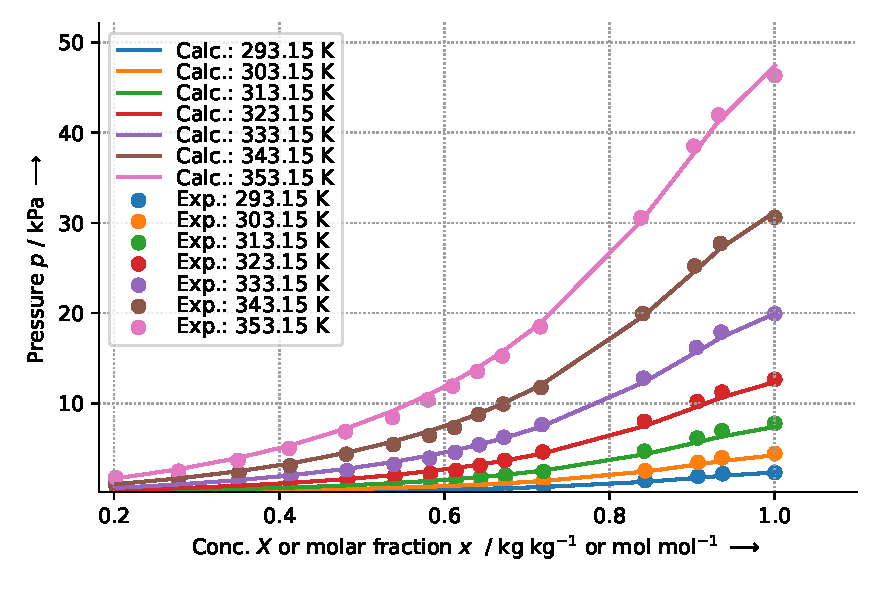
\includegraphics[height=10cm, keepaspectratio]{figs/abs/abs_Water_ionic_liquid_[DEMA][OMs]_NrtlFixedDg_1.pdf}}
\end{figure}
%

To generate the figure, the following refrigerant functions were selected:
\begin{itemize}
\item Vapor pressure: VaporPressure\_EoS1 - ID 1
\item Saturated liquid density: SaturatedLiquidDensity\_EoS1 - ID 1
\end{itemize}

The uncertainity of the experimental data is:
\begin{itemize}
\item Data source $\,\to\,$ Data was taken from table
\item Temperature, absolute, in $\si{\kelvin}$ $\,\to\,$ 0.01
\end{itemize}

The mean absolute percentage error (MAPE) between the experimental and calculated data results in 5.45\%.
\FloatBarrier
\newpage
%%%%%%%%%%%%%%%%%%%%%%%%%%%%%%%%%%%%%%%%%%%%%%%%%%%%%%%%%%%%%%%%%%%%%%%%%%%%%%%
